% Options for packages loaded elsewhere
\PassOptionsToPackage{unicode}{hyperref}
\PassOptionsToPackage{hyphens}{url}
\PassOptionsToPackage{dvipsnames,svgnames,x11names}{xcolor}
%
\documentclass[
  letterpaper,
  DIV=11,
  numbers=noendperiod]{scrreprt}

\usepackage{amsmath,amssymb}
\usepackage{iftex}
\ifPDFTeX
  \usepackage[T1]{fontenc}
  \usepackage[utf8]{inputenc}
  \usepackage{textcomp} % provide euro and other symbols
\else % if luatex or xetex
  \usepackage{unicode-math}
  \defaultfontfeatures{Scale=MatchLowercase}
  \defaultfontfeatures[\rmfamily]{Ligatures=TeX,Scale=1}
\fi
\usepackage{lmodern}
\ifPDFTeX\else  
    % xetex/luatex font selection
\fi
% Use upquote if available, for straight quotes in verbatim environments
\IfFileExists{upquote.sty}{\usepackage{upquote}}{}
\IfFileExists{microtype.sty}{% use microtype if available
  \usepackage[]{microtype}
  \UseMicrotypeSet[protrusion]{basicmath} % disable protrusion for tt fonts
}{}
\makeatletter
\@ifundefined{KOMAClassName}{% if non-KOMA class
  \IfFileExists{parskip.sty}{%
    \usepackage{parskip}
  }{% else
    \setlength{\parindent}{0pt}
    \setlength{\parskip}{6pt plus 2pt minus 1pt}}
}{% if KOMA class
  \KOMAoptions{parskip=half}}
\makeatother
\usepackage{xcolor}
\ifLuaTeX
  \usepackage{luacolor}
  \usepackage[soul]{lua-ul}
\else
  \usepackage{soul}
  
\fi
\setlength{\emergencystretch}{3em} % prevent overfull lines
\setcounter{secnumdepth}{5}
% Make \paragraph and \subparagraph free-standing
\ifx\paragraph\undefined\else
  \let\oldparagraph\paragraph
  \renewcommand{\paragraph}[1]{\oldparagraph{#1}\mbox{}}
\fi
\ifx\subparagraph\undefined\else
  \let\oldsubparagraph\subparagraph
  \renewcommand{\subparagraph}[1]{\oldsubparagraph{#1}\mbox{}}
\fi


\providecommand{\tightlist}{%
  \setlength{\itemsep}{0pt}\setlength{\parskip}{0pt}}\usepackage{longtable,booktabs,array}
\usepackage{calc} % for calculating minipage widths
% Correct order of tables after \paragraph or \subparagraph
\usepackage{etoolbox}
\makeatletter
\patchcmd\longtable{\par}{\if@noskipsec\mbox{}\fi\par}{}{}
\makeatother
% Allow footnotes in longtable head/foot
\IfFileExists{footnotehyper.sty}{\usepackage{footnotehyper}}{\usepackage{footnote}}
\makesavenoteenv{longtable}
\usepackage{graphicx}
\makeatletter
\def\maxwidth{\ifdim\Gin@nat@width>\linewidth\linewidth\else\Gin@nat@width\fi}
\def\maxheight{\ifdim\Gin@nat@height>\textheight\textheight\else\Gin@nat@height\fi}
\makeatother
% Scale images if necessary, so that they will not overflow the page
% margins by default, and it is still possible to overwrite the defaults
% using explicit options in \includegraphics[width, height, ...]{}
\setkeys{Gin}{width=\maxwidth,height=\maxheight,keepaspectratio}
% Set default figure placement to htbp
\makeatletter
\def\fps@figure{htbp}
\makeatother
% definitions for citeproc citations
\NewDocumentCommand\citeproctext{}{}
\NewDocumentCommand\citeproc{mm}{%
  \begingroup\def\citeproctext{#2}\cite{#1}\endgroup}
\makeatletter
 % allow citations to break across lines
 \let\@cite@ofmt\@firstofone
 % avoid brackets around text for \cite:
 \def\@biblabel#1{}
 \def\@cite#1#2{{#1\if@tempswa , #2\fi}}
\makeatother
\newlength{\cslhangindent}
\setlength{\cslhangindent}{1.5em}
\newlength{\csllabelwidth}
\setlength{\csllabelwidth}{3em}
\newenvironment{CSLReferences}[2] % #1 hanging-indent, #2 entry-spacing
 {\begin{list}{}{%
  \setlength{\itemindent}{0pt}
  \setlength{\leftmargin}{0pt}
  \setlength{\parsep}{0pt}
  % turn on hanging indent if param 1 is 1
  \ifodd #1
   \setlength{\leftmargin}{\cslhangindent}
   \setlength{\itemindent}{-1\cslhangindent}
  \fi
  % set entry spacing
  \setlength{\itemsep}{#2\baselineskip}}}
 {\end{list}}
\usepackage{calc}
\newcommand{\CSLBlock}[1]{\hfill\break\parbox[t]{\linewidth}{\strut\ignorespaces#1\strut}}
\newcommand{\CSLLeftMargin}[1]{\parbox[t]{\csllabelwidth}{\strut#1\strut}}
\newcommand{\CSLRightInline}[1]{\parbox[t]{\linewidth - \csllabelwidth}{\strut#1\strut}}
\newcommand{\CSLIndent}[1]{\hspace{\cslhangindent}#1}

\KOMAoption{captions}{tableheading}
\makeatletter
\@ifpackageloaded{tcolorbox}{}{\usepackage[skins,breakable]{tcolorbox}}
\@ifpackageloaded{fontawesome5}{}{\usepackage{fontawesome5}}
\definecolor{quarto-callout-color}{HTML}{909090}
\definecolor{quarto-callout-note-color}{HTML}{0758E5}
\definecolor{quarto-callout-important-color}{HTML}{CC1914}
\definecolor{quarto-callout-warning-color}{HTML}{EB9113}
\definecolor{quarto-callout-tip-color}{HTML}{00A047}
\definecolor{quarto-callout-caution-color}{HTML}{FC5300}
\definecolor{quarto-callout-color-frame}{HTML}{acacac}
\definecolor{quarto-callout-note-color-frame}{HTML}{4582ec}
\definecolor{quarto-callout-important-color-frame}{HTML}{d9534f}
\definecolor{quarto-callout-warning-color-frame}{HTML}{f0ad4e}
\definecolor{quarto-callout-tip-color-frame}{HTML}{02b875}
\definecolor{quarto-callout-caution-color-frame}{HTML}{fd7e14}
\makeatother
\makeatletter
\@ifpackageloaded{bookmark}{}{\usepackage{bookmark}}
\makeatother
\makeatletter
\@ifpackageloaded{caption}{}{\usepackage{caption}}
\AtBeginDocument{%
\ifdefined\contentsname
  \renewcommand*\contentsname{Table of contents}
\else
  \newcommand\contentsname{Table of contents}
\fi
\ifdefined\listfigurename
  \renewcommand*\listfigurename{List of Figures}
\else
  \newcommand\listfigurename{List of Figures}
\fi
\ifdefined\listtablename
  \renewcommand*\listtablename{List of Tables}
\else
  \newcommand\listtablename{List of Tables}
\fi
\ifdefined\figurename
  \renewcommand*\figurename{Figure}
\else
  \newcommand\figurename{Figure}
\fi
\ifdefined\tablename
  \renewcommand*\tablename{Table}
\else
  \newcommand\tablename{Table}
\fi
}
\@ifpackageloaded{float}{}{\usepackage{float}}
\floatstyle{ruled}
\@ifundefined{c@chapter}{\newfloat{codelisting}{h}{lop}}{\newfloat{codelisting}{h}{lop}[chapter]}
\floatname{codelisting}{Listing}
\newcommand*\listoflistings{\listof{codelisting}{List of Listings}}
\makeatother
\makeatletter
\makeatother
\makeatletter
\@ifpackageloaded{caption}{}{\usepackage{caption}}
\@ifpackageloaded{subcaption}{}{\usepackage{subcaption}}
\makeatother
\ifLuaTeX
  \usepackage{selnolig}  % disable illegal ligatures
\fi
\usepackage{bookmark}

\IfFileExists{xurl.sty}{\usepackage{xurl}}{} % add URL line breaks if available
\urlstyle{same} % disable monospaced font for URLs
\hypersetup{
  pdftitle={Viswa Kumar \textbar{} Book Notes for AI Engineering by Chip Huyen},
  pdfauthor={Viswa Kumar},
  colorlinks=true,
  linkcolor={blue},
  filecolor={Maroon},
  citecolor={Blue},
  urlcolor={Blue},
  pdfcreator={LaTeX via pandoc}}

\title{Viswa Kumar \textbar{} Book Notes for AI Engineering by Chip
Huyen}
\author{Viswa Kumar}
\date{2025-02-14}

\begin{document}
\maketitle

\renewcommand*\contentsname{Table of contents}
{
\hypersetup{linkcolor=}
\setcounter{tocdepth}{2}
\tableofcontents
}
\bookmarksetup{startatroot}

\chapter*{Preface}\label{preface}
\addcontentsline{toc}{chapter}{Preface}

\markboth{Preface}{Preface}

Welcome to my book notes website for the book \textbf{AI Engineering by
\emph{Chip Huyen}}. In this website, I have documented all of my notes
for this book, chapter by chapter as I read through the content.

Taking notes from the book you read, not only firms the understanding,
but also serves as a quick summary / reference of the key concepts,
should you wanna look into at a later point in time.

Normally I do this for my safe keeping, but now I'm trying to document
my knowledge journey for the public benefit as well.

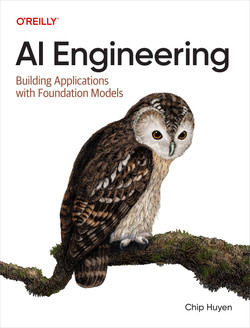
\includegraphics{cover.jpeg}

\begin{tcolorbox}[enhanced jigsaw, leftrule=.75mm, breakable, colframe=quarto-callout-caution-color-frame, bottomrule=.15mm, opacityback=0, arc=.35mm, colback=white, rightrule=.15mm, toprule=.15mm, left=2mm]
\begin{minipage}[t]{5.5mm}
\textcolor{quarto-callout-caution-color}{\faFire}
\end{minipage}%
\begin{minipage}[t]{\textwidth - 5.5mm}

Please don't consider my notes as a \emph{free} replacement to the
actual book. I \ul{strongly encourage you to buy the actual book} to
compensate for all the efforts the author(s) \& publishing house team
put together to deliver the book.

All the actual content of the book are the IPs of the book. I'm merely
recollecting, summarizing \& articulating what I learnt from the book
along with my own thoughts \& opinions.

\end{minipage}%
\end{tcolorbox}

\bookmarksetup{startatroot}

\chapter*{Chapter 1}\label{chapter-1}
\addcontentsline{toc}{chapter}{Chapter 1}

\markboth{Chapter 1}{Chapter 1}

This chapter introduces the term \emph{AI Engineering} and attempts to
define how it is different from \emph{ML Engineering} (which has been
there for many years). First the book introduces very concepts like
language model, large \& frontier models etc and also talks about the
opportunity of AI Engineering.

There are 2 types of language models conceptually 1) Masked models -
Models are trained to predict the fill in the masked words (aka fill in
the blanks). These models are useful for classification, translations
etc. In other words \emph{encoder} heavy 2) Autoregressive models -
Models are trained to predict the next word in the sequence. These
models are useful for text generative tasks such as summarization,
instruction following, chatbots etc. In other words, \emph{decoder}
heavy.

If the model accepts more than 1 data modality (forms of input), they
are \emph{Multi-modal-Model} .

Within the AI Engineering stack, there could be 3 layers
(Infrastructure, Model Development \& Application Development).

The rush and value proposition is on the applications built on top of
foundational models and this book argues that knowing how these models
are trained and the science behind those models would help make several
key long term decisions in choosing, fine-tuning \& tweaking the models
for application needs. The moat is clearly on the application layers
since only handful of large companies can stomach the investments in
doing any groundbreaking research on the model creation itself and
majority of the industry will add value to the application layer.

Before jumping directly to GenAI app development, it is crucial to
define the success. Some possible metrics could be 1) LLM output quality
2) Time To First Token (TTFT), Time Per Output Token (TPOT), Overall
Latency 3) Cost for the APIs 4) Fairness, Consistency, Accuracy etc.

Use model evaluation techniques to deal with the \emph{probablistic}
nature of uncertain LLM outputs to gauge whether you are going in right
direction, is it worth to invest time and effort on this.

Basically an enterprise will jump into AI only for 3 reasons:

\begin{enumerate}
\def\labelenumi{\arabic{enumi})}
\tightlist
\item
  Without AI, the company's main business will be replaced. Eg anything
  that deals heavily with text content - content creation, copyright etc
\item
  Without AI the company will miss lot of value creation. Eg anything
  that can be automated, more productivity with less investment
\item
  Without AI, the company will be left behind while others are bathing
  in shiny light. Eg anything that is more of a GPT wrapper
\end{enumerate}

On the Model development, there are 3 stages

\begin{itemize}
\tightlist
\item
  Pre-Training - activities including gathering training data, cleaning,
  tokenziation, embeddings and generating a foundational model to
  predict the next token effectively
\item
  Post-Training / Fine-Tuning - activities that further train the
  pre-trained model to produce outputs that are aligned to human
  preference
\end{itemize}

For the ML engineering tasks, several training algo exists and for each
task specific labelled dataset is used. ML engineering for the most part
is SFT with labelled data. AI Engg on the other hand deals with
unstructured data and often self supervised fine tuning is employed.
Training to predict the next token is often the only training algorithm
that is employed in AI Engg. Hence for AI Engg, the knowledge of ML
algos are nice to have but not strictly needed. However the skill to
optimize the inference for the hardware is much needed in AI Engg. In
case of ML engg, feature engineering esp with tabular data is needed
whereas in AI Engg, data cleaning, de-duplication, tokenization, context
retrieval etc are more needed.

Another important distinction is \emph{mindshift} . Incase of ML
engineering, one would go from Data -\textgreater{} Model
-\textgreater{} Product. Incase of AI Engg, we go from Product
-\textgreater{} Data -\textgreater{} Model. i.e we use existing models
and try to productize . If that is not solving the problem, we augment
the model with external KB using RAG etc and finally resort to fine tune
the model with custom data, thereby creating a specialized model when
needed.

\bookmarksetup{startatroot}

\chapter*{Chapter 2}\label{chapter-2}
\addcontentsline{toc}{chapter}{Chapter 2}

\markboth{Chapter 2}{Chapter 2}

This chapter starts with Training data. For GPT like LLMs, internet is
the training data. It is impossible to curate a special training data
for LLMs. Hence the approach was to use whatever that was available.
Google's C4 dataset (Colossal Clean Common Crawl) was a refined dataset
from Common Crawl dataset. The dataset is already skewed, biased and
unfairly composed of dominating subjects. English language is unfairly
represented more than other worldly languages, so does with technology
than other useful domains. So naturally the LLMs are more general than
specifically trained for a special purpose domain.

In future, model trainers would have a special arrangement with
publishing houses to seek quality data for pre-training needs. Moving
forward, original content would be even more valuable.

Many model architectures are available but the one that is popular is
Transformer. The journey started with Sequence-to-Sequence, followed by
RNNs and then took a turn in Transformer. Now we have space based models
like Mixture of Experts (MoEs) (\emph{aka Sparse Models}), hybrid
architectures like Mamba, Jamba etc.

Transformer contains Encoder \& Decoder modules. Encoder tries to
capture different dimensions of input token (embedding) into a vector
representations. Decoder tries to probabilistically predict output
tokens based on those internal vector representations. What made
transformer unique is the attention mechanism.

Attention is basically a technique where, when the decoder is trying to
predict the output token, it helps the decoder to help select certain
dimensions of the input tokens such that the output token is making
sense when in the context with input token. i.e While predicting the
output token w.r.t the set of input token, which of the input tokens
should be taken into account? That question is answered by this
attention mechanism.

At a low level, this is done using the KQV matrices. K stands for Key -
for which attention is needed, Q are the queries i.e for the token
pointed by K, what are the tokens that needs to queried \emph{(studied
or should be taken for attention)} and finally V stands for Values i.e
for the tokens pointed by Q, the corresponding Weights are taken as
Values. This values are then multiplied (\emph{looked at}) by the
weights of the actual token (pointed by K) and that is the learning for
the Kth token.

Model designers will need to set some values to decide on the model
architecture

\texttt{d\_model} - model's hidden size \texttt{d\_ff} - feedforward
dimension \texttt{V} - Model's vocab size - list of total words / tokens
that the model may learn \texttt{C} - Position indices to track - this
is related to attention i.e the position of the token as part of the
attention mechanism

Vocab size - the total size of the tokens used in training Context
length - the total length of the model's memory.

All this put together will determine the model's total transformer,
output and other blocks, the total parameter size and the total amount
tokens that needs to be used for training.

Higher the model size (params), 20x times the token is needed for
training. It is not a wrong thing to train a higher size model with
lower tokens but it simply a wasted effort since the training
performance can be achieved with lower size model itself. Hence if you
end up having a higher size model, make sure you train that model with
20x tokens. This is termed as \emph{Scaling Law}

FLOPS - Floating Point Operations FLOP/s - Number of FLOPS per second.
Although it is not clear how one could estimate the number of FLOPS from
the model size / architecture that was decided above. Perhaps the number
of transformer blocks and the associated matmul operations could be used
to estimate the FLOPS?

Parameters are the basically the variables that the model learns during
the training. Weights and Biases. Hyperparameters are the varialble that
one can control. Vocab Size, model dimensions etc. Setting the
hyperparam heavily influence the model performance and hence setting
this right is important and you won't get too many changes since the
training run is costly. Hence there is a new field of research that
extrapolate the performance of small models to tune the hyperparameters
of large models.

In summary, three numbers signal a model's scale: - Number of
parameters, which is a proxy for the model's learning capacity. - Number
of tokens a model was trained on, which is a proxy for how much a model
learned. - Number of FLOPs, which is a proxy for the training cost.

\section*{Post Training :}\label{post-training}
\addcontentsline{toc}{section}{Post Training :}

\markright{Post Training :}

SFT - Supervised finetuning - Fine tune the pre-trained model with a
labelled dataset Preference Finetuning - Further funetune the model to
align the output responses to human preferences. This includes - RLHF :
reinforcement learning with human feedback (llama2) - DPO : direct
preference optimization (llama3)

\subsection*{Typical training
pipleline}\label{typical-training-pipleline}
\addcontentsline{toc}{subsection}{Typical training pipleline}

low quality data -\textgreater{} self supervised finetuning
-\textgreater{} pretrained model -\textgreater{} SFT with labelled data
-\textgreater{} SFT Model -\textgreater{} comparison data with RLHF
-\textgreater{} Reward model -\textgreater{} Prompt engg with reward
model -\textgreater{} final model

\subsection*{RLHF / Preference Fine
tuning}\label{rlhf-preference-fine-tuning}
\addcontentsline{toc}{subsection}{RLHF / Preference Fine tuning}

RLHF uses human labellers / annotaters to reward comparison data. Humans
cannot provide numeric rewards for a given prompt consistently. But they
can pick a best response from given choices. This method is working but
very slow and often expensive.

\section*{Sampling}\label{sampling}
\addcontentsline{toc}{section}{Sampling}

\markright{Sampling}

This is also called as \emph{Un Embedding Layer} . Sampling is basically
choosing the best output from available samples. When the model predicts
the next token, it produces a \emph{logit} vector. In case of
classification task, the logic vector simply 2 dimensions (yes/no)
(spam/not spam) . Each element of the vector contains a probability of
that class. i.e yes 90*, no 10\% etc. In reality the logic vector
contains the learned weights of the corresponding output token, which
then sent via \emph{Softmax} layer to convert that weight to
probability.

For language model, the probabilistic vector works differently. In this
case, the \emph{logic} vector contains the vocab size dimension. i.e if
the vocab size is 50,256, there would 50,2056 elements in the vector
with a probability for each token. i.e \texttt{logit{[}245{]}\ =\ 0.10}
would simply mean 245th token (could something like \texttt{t})'s
probability is 10\%.

In language model, simply the most probable token won't be useful.
Because if that's the case, you will always be seeing same output
without any context based on the probability of the token patterns seen
during the training phase. Instead for the language models, the
probability is used as the probability of selecting that output token.
i.e For example if the logit of \texttt{a} is \texttt{0.9} and
\texttt{t} is \texttt{0.1}, then the output \texttt{t} will be chosen
for 10\% of the time and the output \texttt{a} will be chosen for 90\%
of the time, so on so forth.

And because there are too many logit elements on the logit vector due to
sheer size of voab size, instead of doing probabilities on the
\emph{softmax} on the vector, it is done as \emph{logprobs} i.e output
probabilities are converted into logarithmic scale and then the
probabilities are applied.

There are several other strategies used to sample the output token from
those probabilities

\begin{enumerate}
\def\labelenumi{\arabic{enumi})}
\tightlist
\item
  Temperature - higher the value, more rare tokens are selected than
  more obvious tokens. This basically achieved by dividing the
  probability value by this temperature (\texttt{Xi/T}) so that it
  elevates the probability of less value tokens.
\item
  Top-k - Instead of taking the entire vocab dimension of the logit
  vector and computing the probabilities, select the top K elements and
  then do the probability calculation, thereby reducing the compute
  load.
\item
  Top-p - Also known as nucleus sampling, instead of selecting the top K
  samples, select the list of tokens that cumulatively satisfies the top
  p.~If p is 90\% (0.9) and if token \texttt{a} is 89\% and \texttt{t}
  is 1\%, then only these 2 tokens are selected.
\item
  Stopping Condition - Give a total token count to stop sampling or use
  a special token like eos, stop word to stop sampling.
\end{enumerate}

\subsection*{Test Time Compute}\label{test-time-compute}
\addcontentsline{toc}{subsection}{Test Time Compute}

The process of selecting the whole output for a completion task. The
more the compute, the more token it can generate. Generating multiple
responses for a single query often improves overall model performance
but comes with the inference cost. This is the \texttt{choices\ {[}{]}}
seen at the OpenAI completions API response. OpenAI found that the model
performance plateaued at 400 outputs mark. i.e if the number of outputs
is \textgreater{} 400, it doesn't contribute to the model performance.
Also to ensure accuracy, these multiple outputs can used to select the
most consistent output as the accurate output.

\subsection*{Structured Output}\label{structured-output}
\addcontentsline{toc}{subsection}{Structured Output}

Structured output can be achieved through 1) prompt engineering with
examples - this often works but not always guaranteed 2) post processing
- certain mistakes can be handled such as missing a \{\} or json output
cutoff due to context length etc. 3) constrained sampling - Need model
knowledge and the ability to influence the sampling using filter of
accepted tokens 4) fine tuning - most expensive but most reliable way to
train a model to output structured outputs

\section*{Probabilistic Nature of
LLM}\label{probabilistic-nature-of-llm}
\addcontentsline{toc}{section}{Probabilistic Nature of LLM}

\markright{Probabilistic Nature of LLM}

2 main problems with this nature

\begin{enumerate}
\def\labelenumi{\arabic{enumi})}
\tightlist
\item
  Inconsistent / Indeterministic output for the sample input / slightly
  different input

  \begin{enumerate}
  \def\labelenumii{\arabic{enumii})}
  \tightlist
  \item
    Use caching as interim solution
  \item
    Use prompt engineering and memory systems
  \end{enumerate}
\item
  Hallucination - where the model generates its own facts not grounded
  in truth. This probably happens due to the fact that the model cannot
  distinguish between the training data and the data that it generates.

  \begin{enumerate}
  \def\labelenumii{\arabic{enumii})}
  \tightlist
  \item
    How a model learns to produce its own data? 2 school of thoughts

    \begin{enumerate}
    \def\labelenumiii{\arabic{enumiii})}
    \tightlist
    \item
      It happens during RLHF if the human annotaters are training the
      model with knowledge that the model doesn't know during training.
      This teaches the model that it is ok to generate new facts that
      are not seen in training
    \item
      The model knows that it generating hallucinating response but it
      still do it because it was told not to do so. Some try to mitigate
      by adding ``Answer Truthfully'' ``if you are unsure say I don't
      know'' in system prompts.
    \end{enumerate}
  \end{enumerate}
\end{enumerate}

The two hypotheses discussed complement each other. The self-delusion
hypothesis focuses on how self-supervision causes hallucinations,
whereas the mismatched internal knowledge hypothesis focuses on how
supervision causes hallucinations.

It is very hard to detect hallucinations in a generic fashion unless we
know for sure the output is not in any training data.

Research tasks:

\begin{itemize}
\tightlist
\item[$\square$]
  How to determine the context length based on the model size /
  architecture?
\item[$\square$]
  How to estimate FLOPS from the model size / architecture?
\item[$\square$]
  How is the test time compute difference from prompting the LLM with
  same prompt again \& again.
\end{itemize}

\bookmarksetup{startatroot}

\chapter*{Chapter 3}\label{chapter-3}
\addcontentsline{toc}{chapter}{Chapter 3}

\markboth{Chapter 3}{Chapter 3}

Coming Soon\ldots{}

\bookmarksetup{startatroot}

\chapter*{Chapter 4}\label{chapter-4}
\addcontentsline{toc}{chapter}{Chapter 4}

\markboth{Chapter 4}{Chapter 4}

Coming Soon\ldots{}

\bookmarksetup{startatroot}

\chapter*{Chapter 5}\label{chapter-5}
\addcontentsline{toc}{chapter}{Chapter 5}

\markboth{Chapter 5}{Chapter 5}

Coming Soon\ldots{}

\bookmarksetup{startatroot}

\chapter*{Chapter 6}\label{chapter-6}
\addcontentsline{toc}{chapter}{Chapter 6}

\markboth{Chapter 6}{Chapter 6}

Coming Soon\ldots{}

\bookmarksetup{startatroot}

\chapter*{Chapter 7}\label{chapter-7}
\addcontentsline{toc}{chapter}{Chapter 7}

\markboth{Chapter 7}{Chapter 7}

Coming Soon\ldots{}

\bookmarksetup{startatroot}

\chapter*{Chapter 8}\label{chapter-8}
\addcontentsline{toc}{chapter}{Chapter 8}

\markboth{Chapter 8}{Chapter 8}

Coming Soon\ldots{}

\bookmarksetup{startatroot}

\chapter*{Chapter 9}\label{chapter-9}
\addcontentsline{toc}{chapter}{Chapter 9}

\markboth{Chapter 9}{Chapter 9}

Coming Soon\ldots{}

\bookmarksetup{startatroot}

\chapter*{Chapter 10}\label{chapter-10}
\addcontentsline{toc}{chapter}{Chapter 10}

\markboth{Chapter 10}{Chapter 10}

Coming Soon\ldots{}

\bookmarksetup{startatroot}

\chapter*{Book Summary}\label{book-summary}
\addcontentsline{toc}{chapter}{Book Summary}

\markboth{Book Summary}{Book Summary}

Coming soon\ldots{}

\bookmarksetup{startatroot}

\chapter*{References}\label{references}
\addcontentsline{toc}{chapter}{References}

\markboth{References}{References}

\phantomsection\label{refs}
\begin{CSLReferences}{0}{1}
\end{CSLReferences}



\end{document}
